% -*- coding: utf-8 -*-
% Структура дисплеев
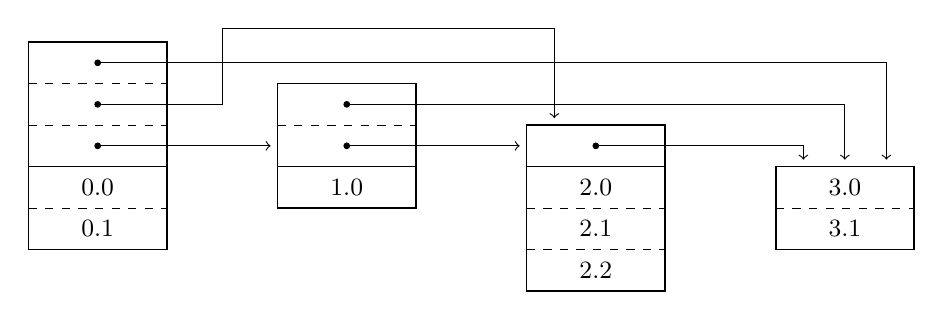
\begin{tikzpicture}
  \tikzstyle{every node}=[font=\small]

  \draw [semithick] (0.0em,  4.5em) rectangle (5.0em, -3.0em);
  \draw [dashed]    (0.0em,  3.0em) -- (5.0em, 3.0em);
  \draw [dashed]    (0.0em,  1.5em) -- (5.0em, 1.5em);
  \draw             (0.0em,  0.0em) -- (5.0em, 0.0em);
  \draw             (2.5em, -0.1em) node[below] {\ic{0.0}};
  \draw [dashed]    (0.0em, -1.5em) -- (5.0em, -1.5em);
  \draw             (2.5em, -1.6em) node[below] {\ic{0.1}};

  \draw [semithick] ( 9.0em,  3.0em) rectangle (14.0em, -1.5em);
  \draw [dashed]    ( 9.0em,  1.5em) -- (14.0em, 1.5em);
  \draw             ( 9.0em,  0.0em) -- (14.0em, 0.0em);
  \draw             (11.5em, -0.1em) node[below] {\ic{1.0}};

  \draw [semithick] (18.0em,  1.5em) rectangle (23.0em, -4.5em);
  \draw             (18.0em,  0.0em) -- (23.0em, 0.0em);
  \draw             (20.5em, -0.1em) node[below] {\ic{2.0}};
  \draw [dashed]    (18.0em, -1.5em) -- (23.0em, -1.5em);
  \draw             (20.5em, -1.6em) node[below] {\ic{2.1}};
  \draw [dashed]    (18.0em, -3.0em) -- (23.0em, -3.0em);
  \draw             (20.5em, -3.1em) node[below] {\ic{2.2}};

  \draw [semithick] (27.0em,  0.0em) rectangle (32.0em, -3.0em);
  \draw             (29.5em, -0.1em) node[below] {\ic{3.0}};
  \draw [dashed]    (27.0em, -1.5em) -- (32.0em, -1.5em);
  \draw             (29.5em, -1.6em) node[below] {\ic{3.1}};


  \filldraw  (2.5em, 3.75em) circle(1.0pt);
  \filldraw  (2.5em, 2.25em) circle(1.0pt);
  \filldraw  (2.5em, 0.75em) circle(1.0pt);
  \draw [->] (2.5em, 3.75em) -- (31.0em, 3.75em) -- (31.0em, 0.25em);
  \draw [->] (2.5em, 2.25em) -- (7.0em, 2.25em) -- (7.0em, 5.0em) --
               (19.0em, 5.0em) -- (19.0em, 1.75em);
  \draw [->] (2.5em, 0.75em) -- (8.75em, 0.75em);

  \filldraw  (11.5em, 2.25em) circle(1.0pt);
  \filldraw  (11.5em, 0.75em) circle(1.0pt);
  \draw [->] (11.5em, 2.25em) -- (29.5em, 2.25em) -- (29.5em, 0.25em);
  \draw [->] (11.5em, 0.75em) -- (17.75em, 0.75em);

  \filldraw  (20.5em, 0.75em) circle(1.0pt);
  \draw [->] (20.5em, 0.75em) -- (28.0em, 0.75em) -- (28.0em, 0.25em);

\end{tikzpicture}
